\chapter{Reliable Broadcast}

\section{Links (unassessed)}
A link is a mechanism defining how two processes may interact by sending and receiving messages, and what properties hold for message passing.

\begin{definitionbox}{Fair Loss Link}
    A weak link abstraction from which other links (e.g stubborn) can be built.
    \begin{center}
        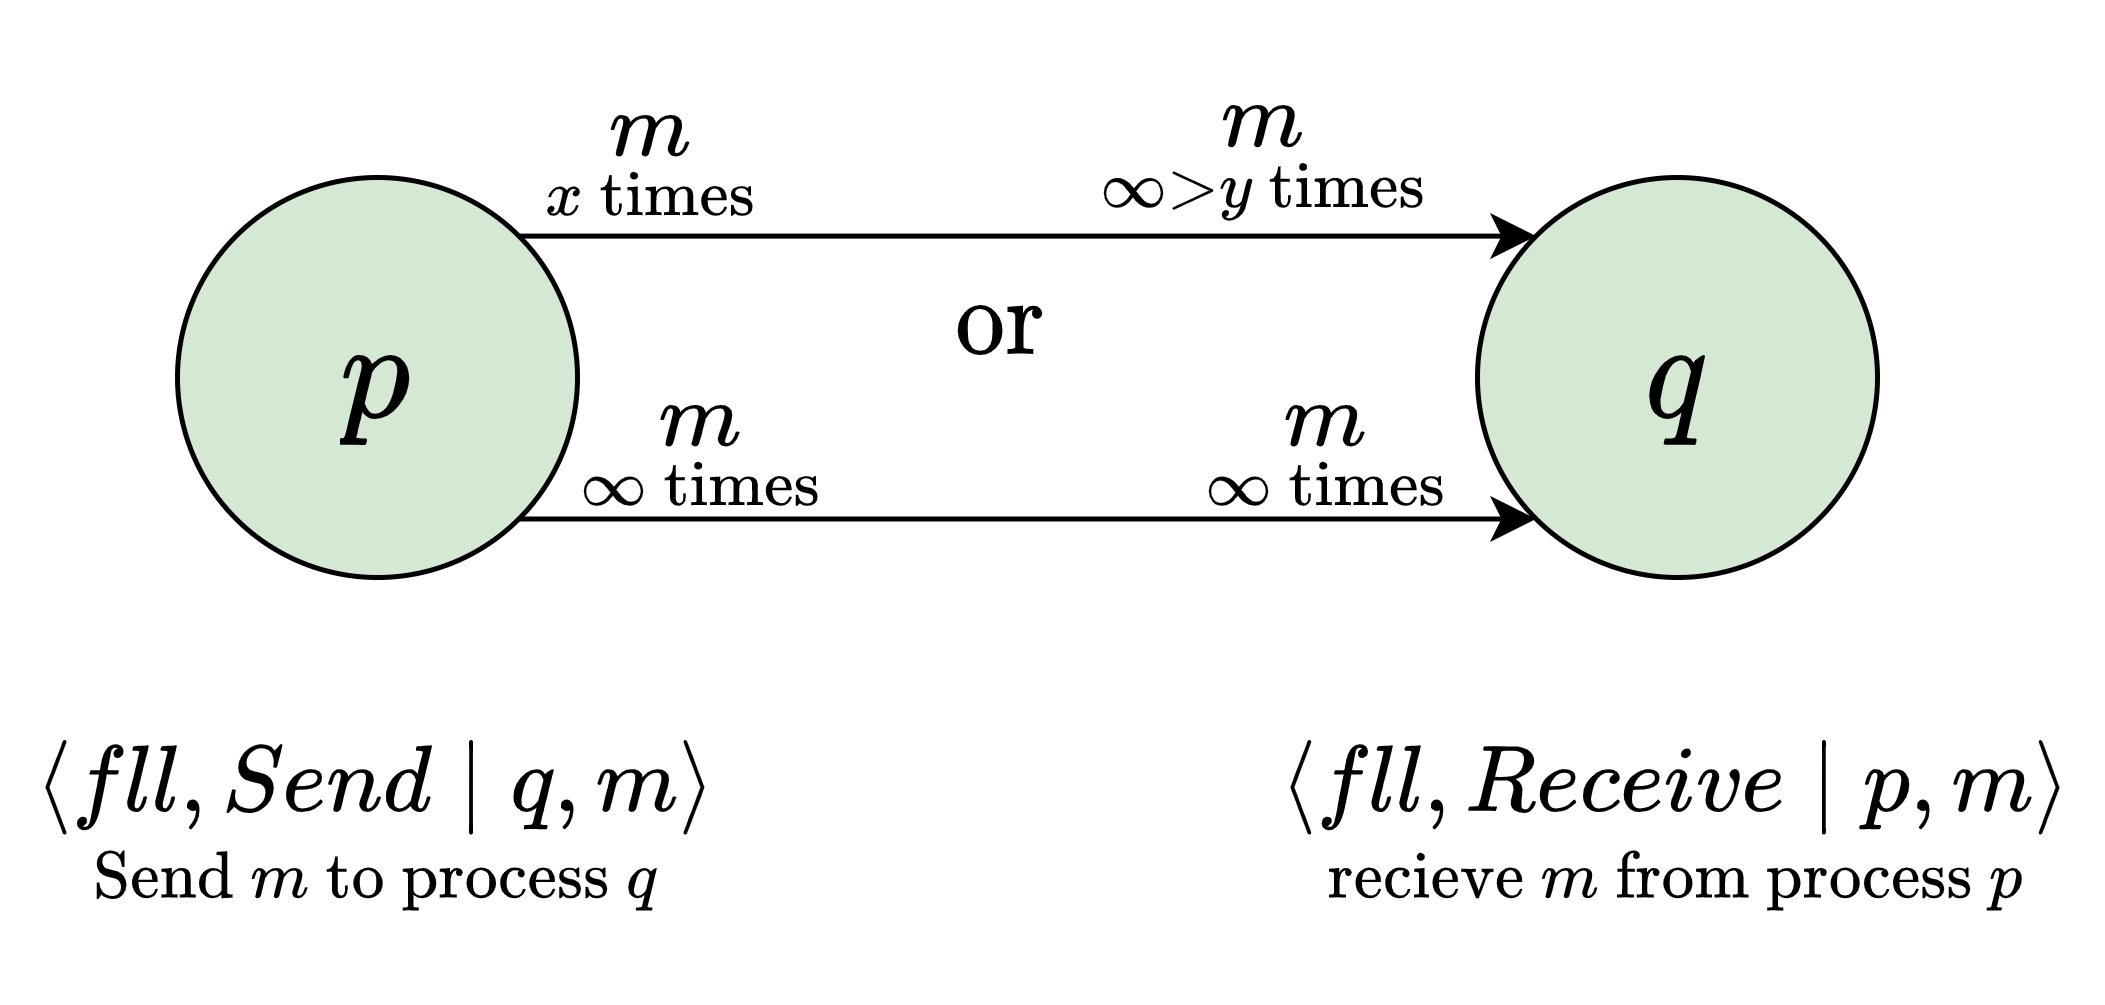
\includegraphics[width=.6\textwidth]{reliable_broadcast/images/fair_loss_links.drawio.png}
    \end{center}
    \begin{tabular}{l l p{.6\textwidth}}
        \textbf{Fair-Loss} & Liveness & Correct process $p$ infinitely sends message $m$ to correct process $q$ $\Rightarrow$ $q$ receives $m$ from $p$ infinitely many times. \\
        \textbf{Finite Duplication} & Liveness & Correct process $p$ sends message $m$ a finite number of times to $q$ $\Rightarrow$ $m$ cannot be received infinitely many times from $p$. \\
        \textbf{No Creation} & Safety & Some process $q$ receives a message $m$ with sender $p$ $\Rightarrow$ $p$ previously sent $m$ to $q$. \\
    \end{tabular}
\end{definitionbox}
\begin{definitionbox}{Stubborn Link}
    A link guaranteeing messages are received infinitely many times.
    \begin{center}
        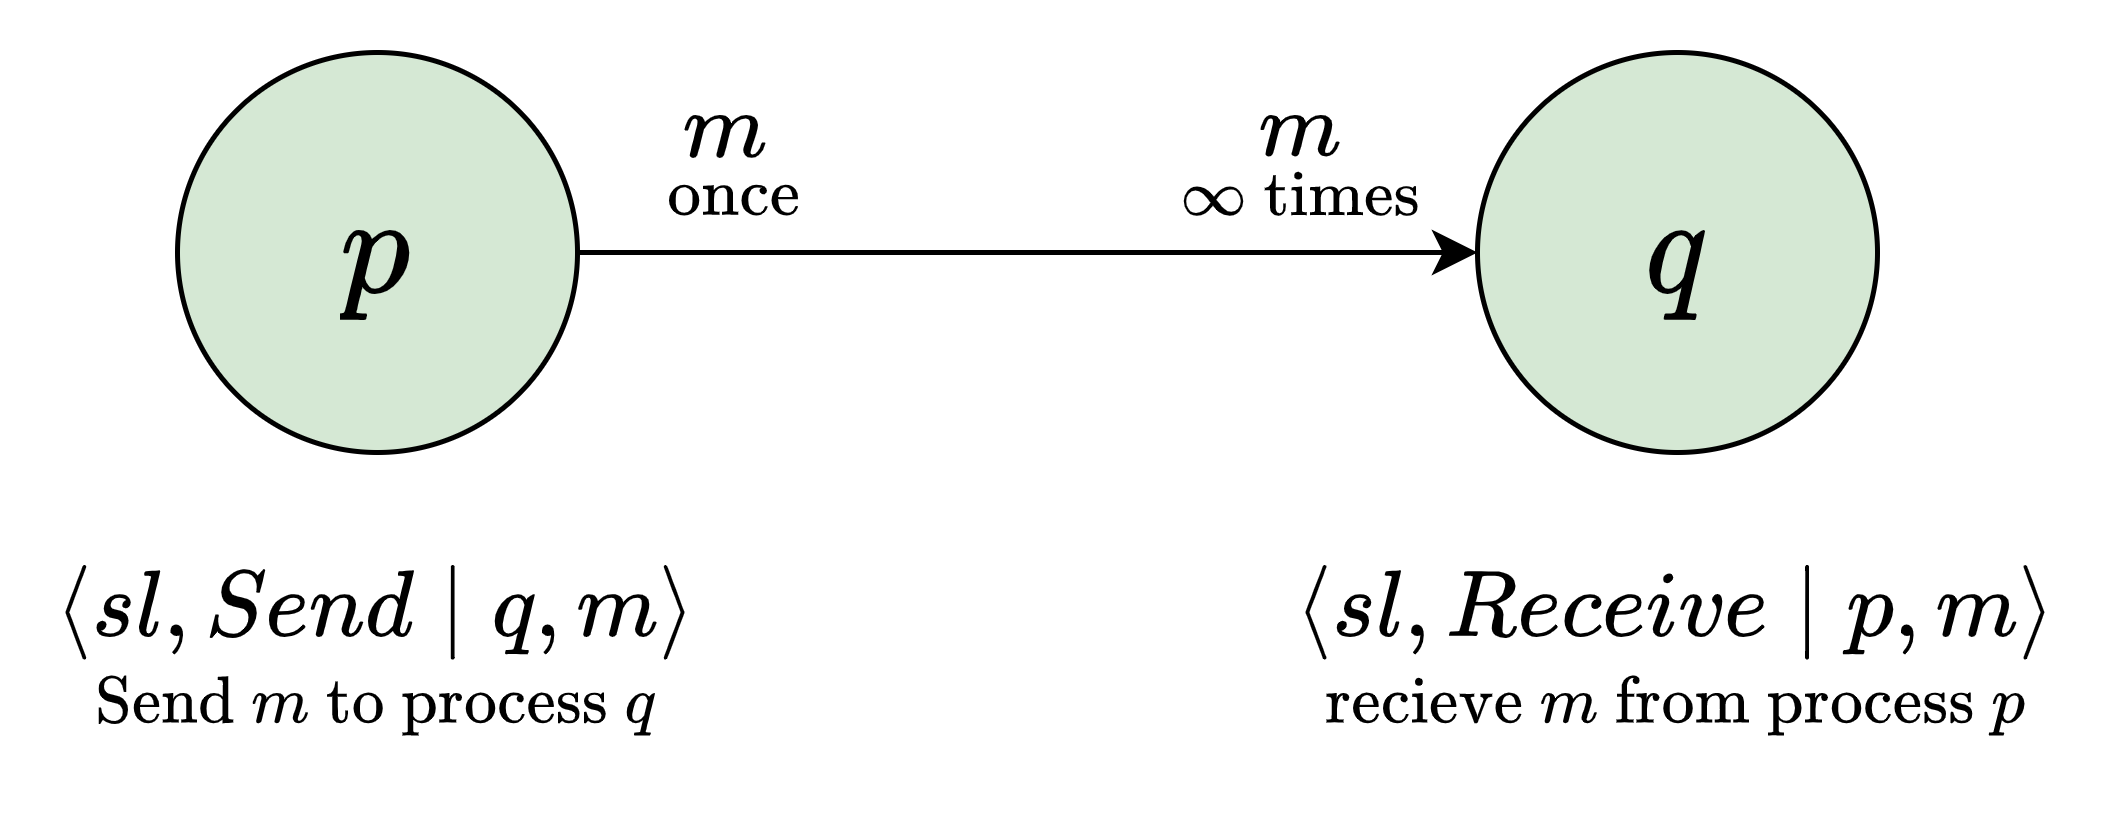
\includegraphics[width=.6\textwidth]{reliable_broadcast/images/stubborn_links.drawio.png}
    \end{center}
    \begin{center}
        \begin{tabular}{l l p{.6\textwidth}}
            \textbf{Stubborn Delivery} & Liveness & Correct process $p$ sends message $m$ to correct process $q$ $\Rightarrow$ $q$ receives $m$ from $p$ infinitely many times. \\
            \textbf{No Creation} & Safety & Some process $q$ receives a message $m$ with sender $p$ $\Rightarrow$ $p$ previously sent $m$ to $q$. \\
        \end{tabular}
    \end{center}
\end{definitionbox}

\begin{examplebox}{No change in mind}
    Implement stubborn links with elixir using the fair loss link.
    \tcblower
    
\end{examplebox}

\begin{definitionbox}{Perfect Point-to-Point Link}
    \begin{center}
        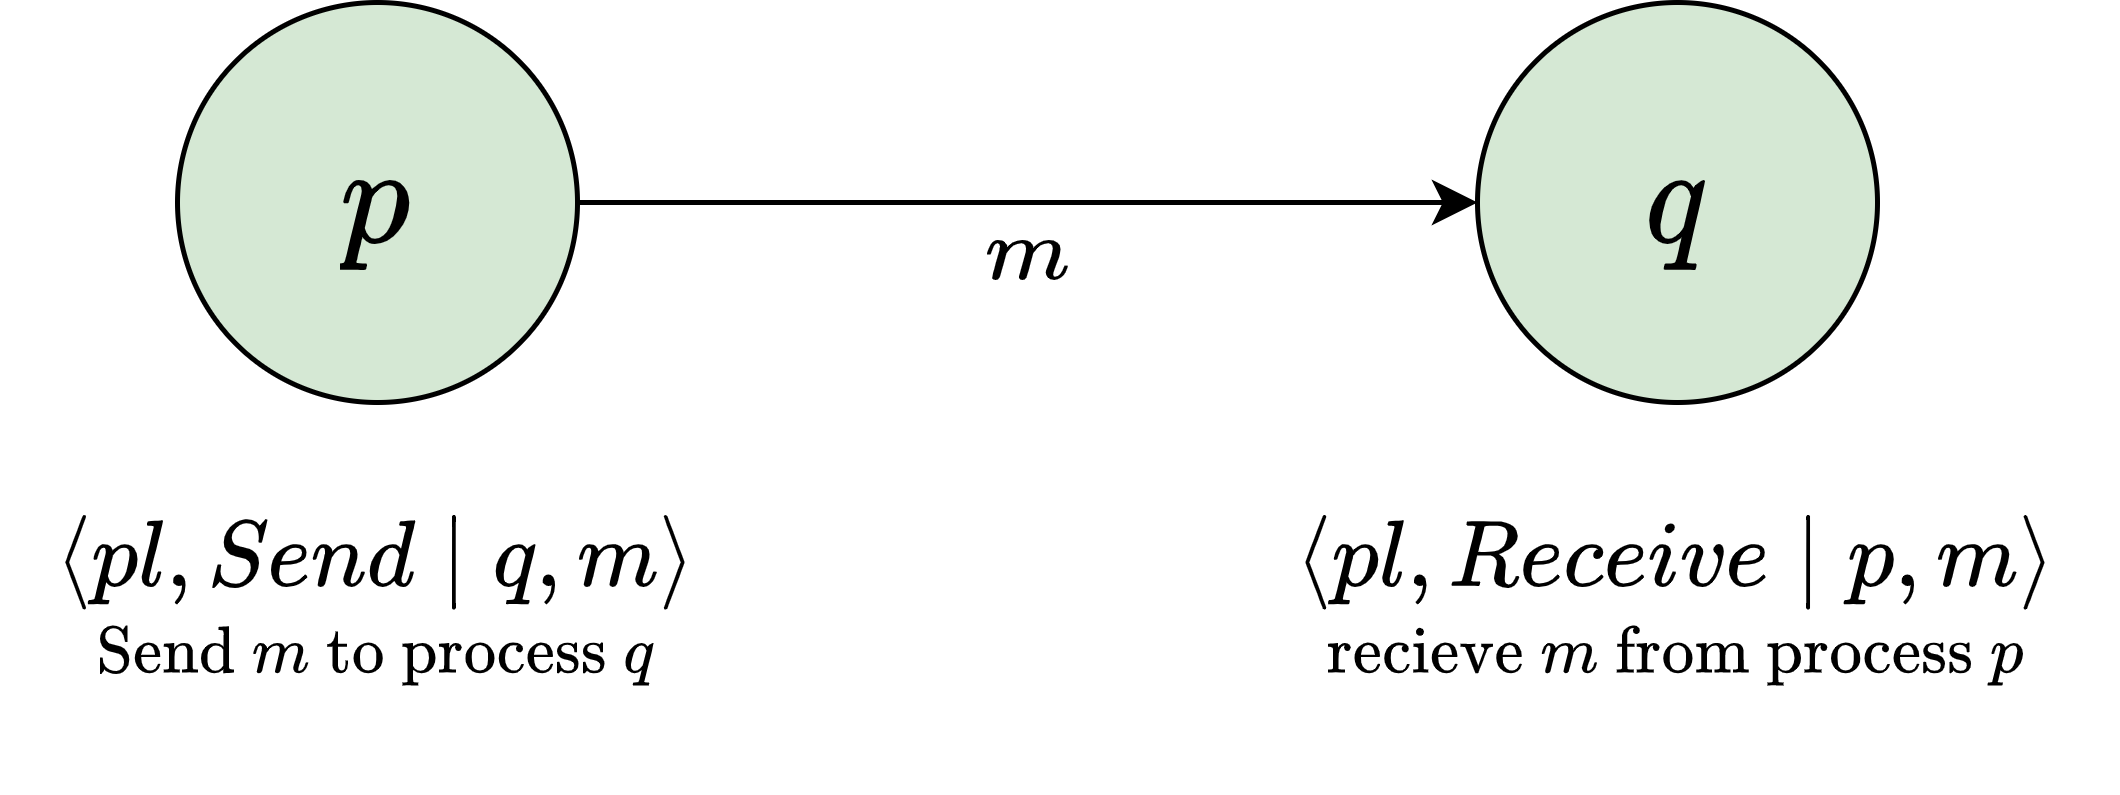
\includegraphics[width=.6\textwidth]{reliable_broadcast/images/perfect_links.drawio.png}
    \end{center}
    \begin{itemize}
        \item Also called \textit{reliable message passing}
    \end{itemize}
    \begin{center}
        \begin{tabular}{l l p{.6\textwidth}}
            \textbf{Reliable Delivery} & Liveness & Correct process $p$ sends $m$ to correct process $q$ $\Rightarrow$ $q$ will eventually receive $m$. \\
            \textbf{No Duplication} & Safety & No message is received by a process more than once. \\
            \textbf{No Creation} & Safety & Some process $q$ receives a message $m$ with sender $p$ $\Rightarrow$ $p$ previously sent $m$ to $q$. \\
        \end{tabular}
    \end{center}
\end{definitionbox}

\section{Failure Detection}
A failure detector provides a process with a list of \textit{suspected processes}.
\begin{itemize}
  \item Failure detectors make, and encapsulate some timing assumptions in order to determine which processes are suspect.
  \item They are not fully accurate, and their specification allows for this.
\end{itemize}

\begin{definitionbox}{Perfect Failure Detector}
  A failure detector that is never incorrect / is entirely accurate.
  \begin{itemize}
    \item Never changes its view on failure $\to$ once detected as crashed it cannot be \textit{unsuspected}.
    \item Often represented as $\mathcal{P}$
  \end{itemize}
  \begin{center}
    \begin{tabular}{l l p{.6\textwidth}}
      \textbf{Strong Completeness} & Liveness & Eventually every process that crashes is permanently detected as crashed by every correct process. \\
      \textbf{Strong Accuracy} & Safety & $p$ detected $\Rightarrow$ $p$ has crashed. No process is suspected before it crashed. \\
    \end{tabular}
\end{center}
\end{definitionbox}

We can implement a failure detector using timeouts and a heartbeat.
\begin{itemize}
  \item Perfect links used to send requests for heartbeat.
  \item If reply is not received before timeout, the process is suspected to have crashed.
  \item \textbf{perfect links} are only reliable for correct processes.
  \item Timeout period has to be long enough to send the heartbeat to all processes and for the receiving processes to respond. 
\end{itemize} 
\inputminted{elixir}{reliable_broadcast/code/perfect_failure_detector.ex}

This implementation meets the properties of a \textit{perfect failure detector} as:
\begin{center}
  \begin{tabular}{l p{.8\textwidth}}
    \textbf{Strong Completeness} & {If a process crashes it will no longer reply to heartbeat messages, 
    hence by \textit{perfect links} \textbf{no-creation} property, no correct process will receive 
    a heartbeat. So every correct process will detect a crash. } \\
    \textbf{Strong Accuracy} & A process can only miss the timeout if it has crashed under out timing assumption.
  \end{tabular}
\end{center}

\begin{definitionbox}{Eventually Perfect Failure Detector}
  A failure detector that is not entirely accurate.
  \begin{itemize}
    \item Can restore processes (no longer suspected).
    \item Often represented as $ \lozenge  \mathcal{P}$
  \end{itemize}
  \begin{center}
    \begin{tabular}{l l p{.6\textwidth}}
      \textbf{Strong Completeness} & Liveness & Eventually every process that crashes is permanently detected as crashed by every correct process.  \\
      \textbf{Eventual Strong Accuracy} & Liveness & Eventually no correct process is suspected by any other correct process \\
    \end{tabular}
\end{center}
\end{definitionbox}

\section{Best Effort Broadcast}
\begin{definitionbox}{Best Effort Broadcast}
    A non-reliable, single-shot broadcast.
    \begin{itemize}
        \item Only reliable if the broadcasting process is correct during broadcast (if crashing during broadcast only some messages may be delivered, and processes may disagree on delivery)
        \item No delivery agreement guarantee (correct processes may disagree on delivery)
        \item Uses \textit{Perfect Point-to-Point Link} and inherits properties from it.
    \end{itemize} 
    \begin{center}
        \begin{tabular}{l l p{.6\textwidth}}
            \textbf{Validity} & Liveness & If a correct process broadcasts a message then every correct process eventually receives it. \\
            \textbf{No Duplication} & Safety & No message is received by a process more than once. \\
            \textbf{No Creation} & Safety & No broadcast is delivered unless it was broadcast. \\
        \end{tabular}
    \end{center}
\end{definitionbox}
We can implement this in elixir using the send and receive primitives as \textit{Perfect Point-to-Point Link}.

\inputminted{elixir}{reliable_broadcast/code/perfect_point_to_point_links.ex}

\section{Reliable Broadcast}
\begin{definitionbox}{Reliable Broadcast}
    Adds a delivery guarantee to \textit{best effort broadcast}  
    \begin{center}
        \begin{tabular}{l l p{.6\textwidth}}
            \textbf{Agreement} & Liveness & If a correct process delivers message $m$ then all correct processes deliver $m$ \\
            \multicolumn{3}{c}{\textbf{All Properties from Best Effort Broadcast}} \\
        \end{tabular}
    \end{center}
    The combination of \textbf{Validity} and \textbf{Agreement} form a \textit{termination property} (system reaches agreement in finite time).
\end{definitionbox}
\begin{center}
  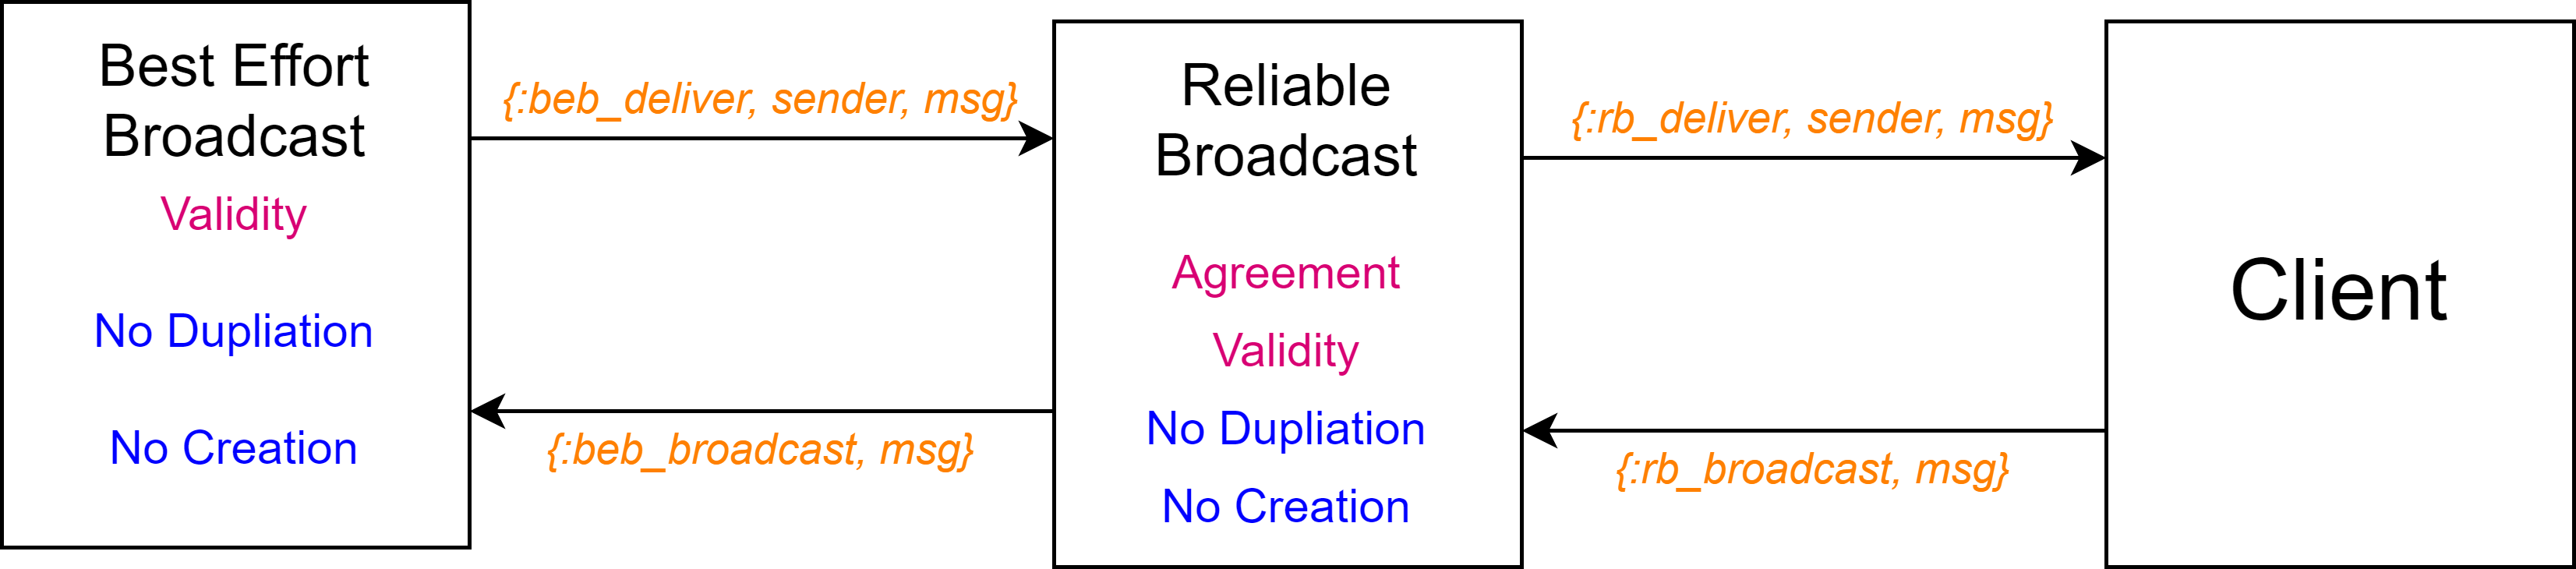
\includegraphics[width=.8\textwidth]{reliable_broadcast/images/reliable_broadcast.drawio.png}
\end{center}

\subsection{Eagre Reliable Broadcast}
\begin{definitionbox}{Eagre Reliable Broadcast}
    A \textit{reliable broadcast} where every process re-broadcasts every message it delivers.
    \begin{itemize}
        \item If the broadcasting process crashes, and only some correct processes deliver the message, then re-broadcast ensures eventually all will receive.
        \item This broadcast is \textit{fail-silent}
        \item Very inefficient to implement, broadcast to $n$ processes results in $O(n^2)$ messages.
        \item \textbf{Validity} property combined with retransmission provides \textbf{agreement}.
    \end{itemize}
    \begin{center}
        \begin{tabular}{l l p{.6\textwidth}}
            \multicolumn{3}{c}{\textbf{All Properties from Reliable Broadcast}} \\
        \end{tabular}
    \end{center}
\end{definitionbox}

\inputminted{elixir}{reliable_broadcast/code/eagre_reliable_broadcast.ex}

\subsection{Lazy Reliable Broadcast}
\begin{definitionbox}{Lazy Reliable Broadcast}
    A \textit{reliable broadcast} using \textit{Best Effort Broadcast} with a \textit{Failure Detector} to enforce agreement.
    \begin{itemize}
        \item Uses a \textit{perfect failure detector}.
        \item When a process is detected to have crashed, all broadcasts delivered from the process are rebroadcasted
        \item Agreement is derived from the \textbf{validity} of \textit{best effort broadcast}, that every correct process broadcasts every message delivered from a crashed process and the properties of the \textit{perfect failure detector}.
    \end{itemize}
\end{definitionbox}

\begin{center}
  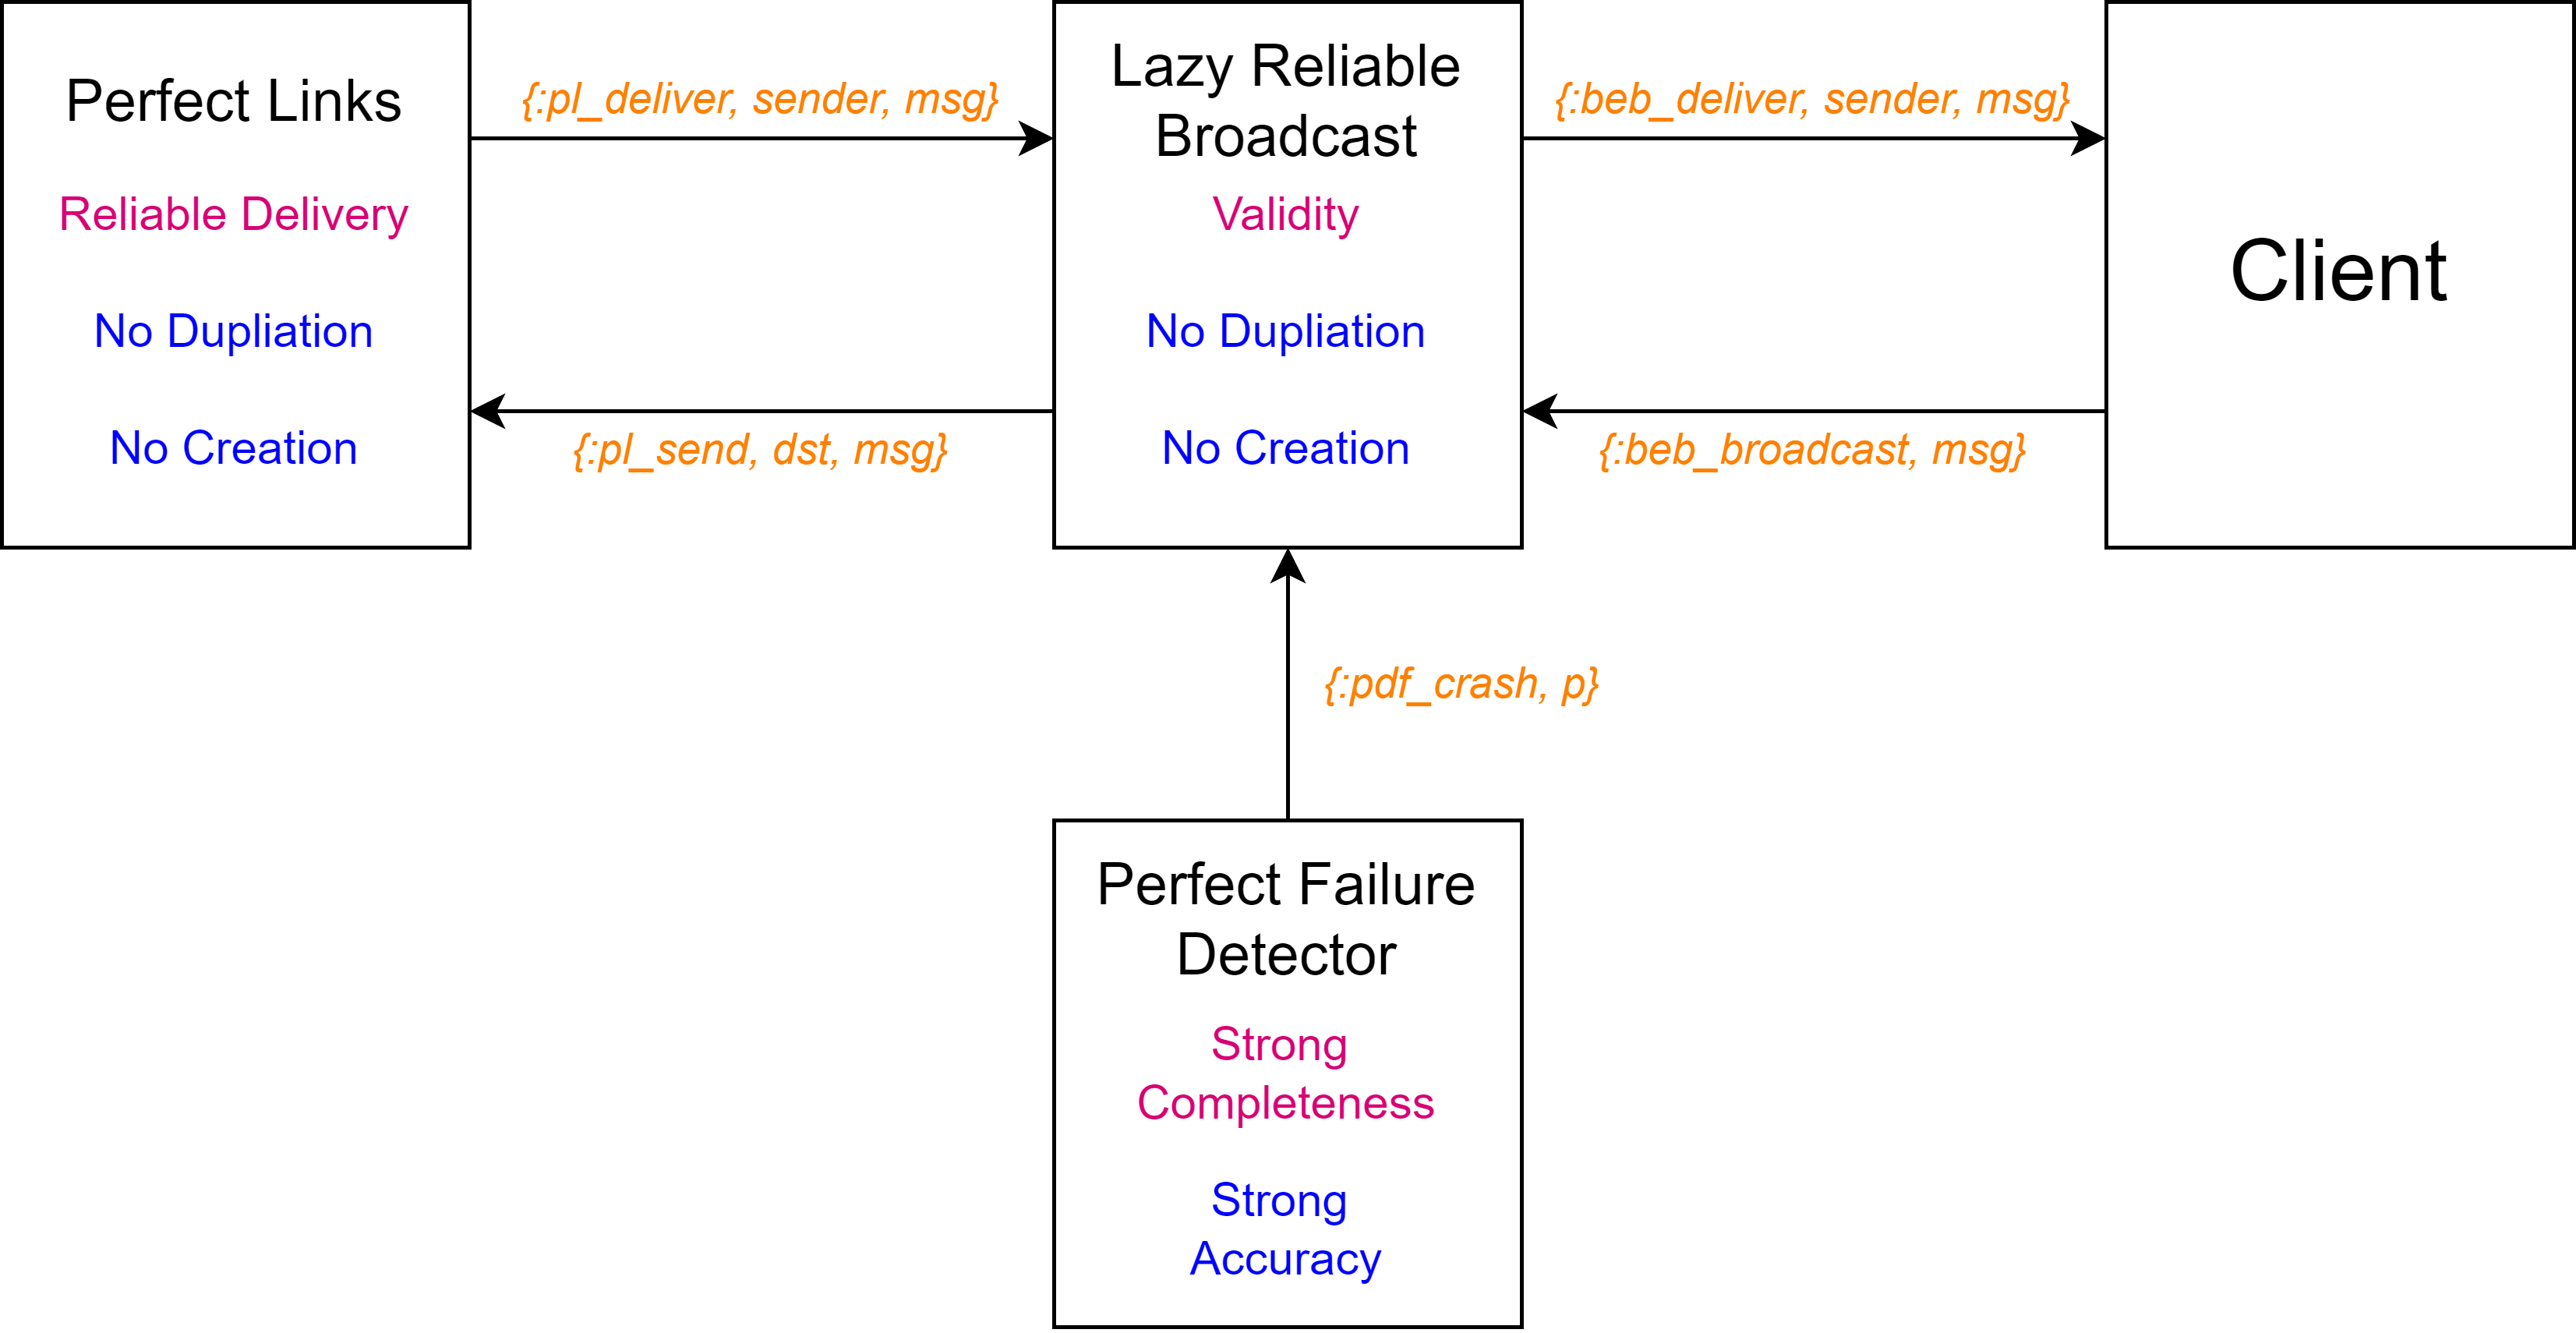
\includegraphics[width=.8\textwidth]{reliable_broadcast/images/lazy_reliable_broadcast.drawio.png}
\end{center}

\inputminted{elixir}{reliable_broadcast/code/lazy_reliable_broadcast.ex}

\section{Uniform Reliable Broadcast}
\begin{definitionbox}{Uniform Reliable Broadcast}
    \begin{center}
        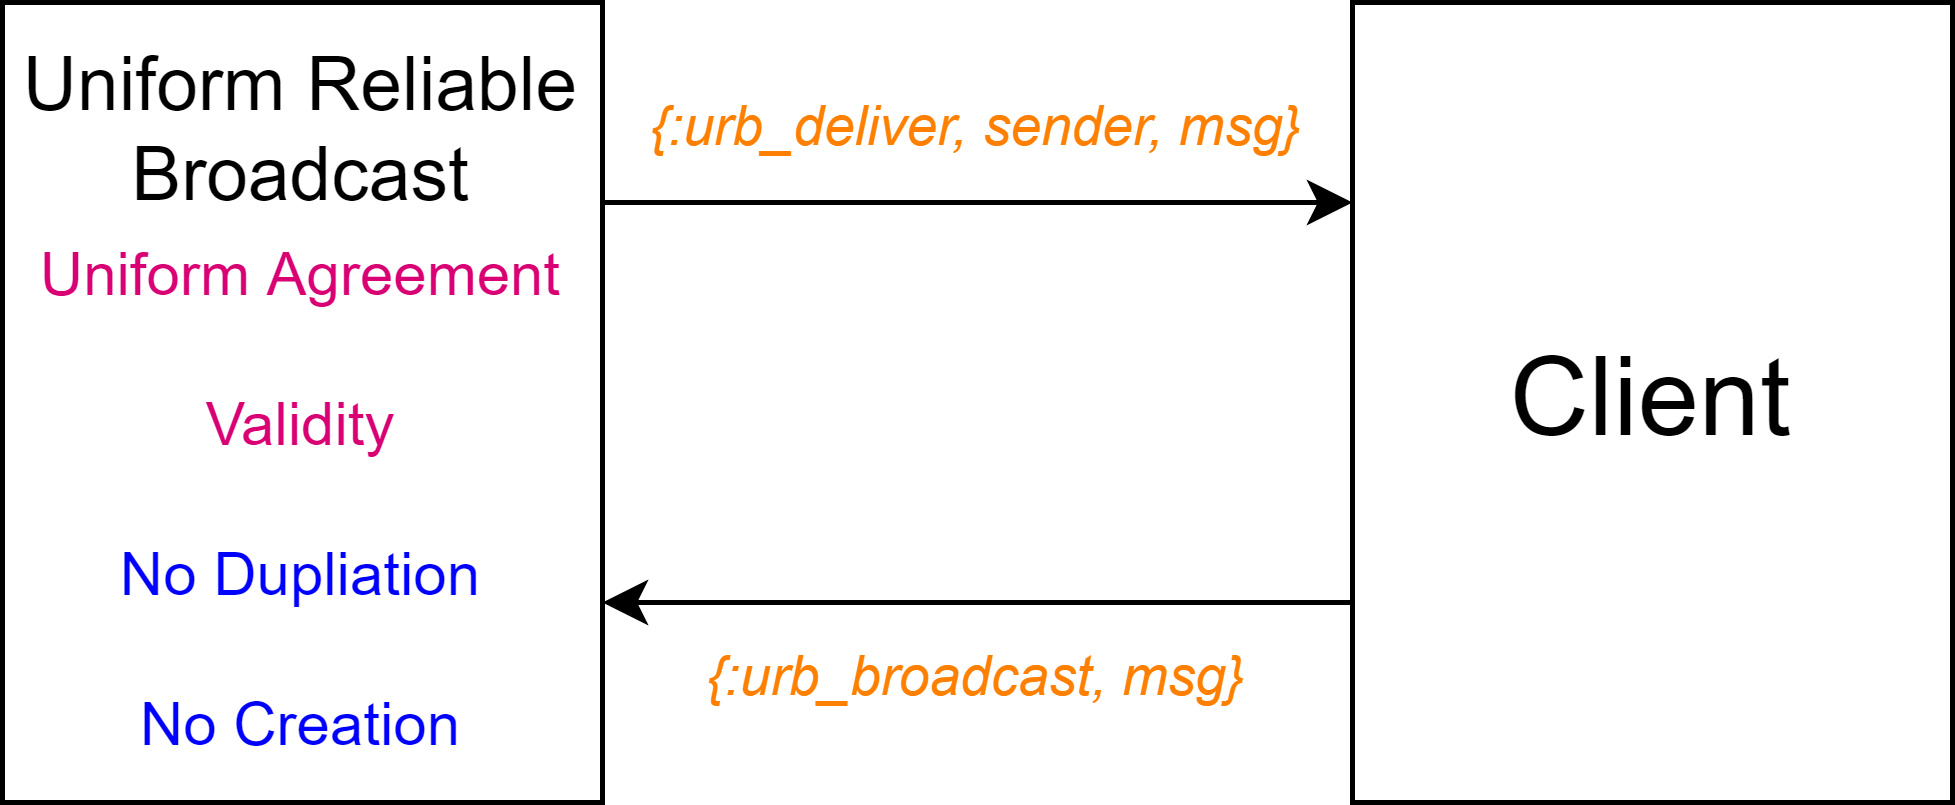
\includegraphics[width=.6\textwidth]{reliable_broadcast/images/uniform_reliable_broadcast.drawio.png}
    \end{center}
    \begin{center}
        \begin{tabular}{l l p{.6\textwidth}}
            \textbf{Uniform Agreement} & Liveness & If a non-correct process delivers message $m$ then all correct processes deliver $m$ \\
            \multicolumn{3}{c}{\textbf{All Properties from Best Effort Broadcast}} \\
        \end{tabular}
    \end{center}
    \begin{itemize}
        \item Implies that faulty processes deliver a subset of messages delivered to correct processes (stronger than \textbf{agreement} - only for correct processes).
        \item Avoids any scenario where a crashed process broadcasts and only a crashed process delivers (correct processes miss message).
    \end{itemize}
\end{definitionbox}

\begin{definitionbox}{Majority Ack Uniform Reliable Broadcast}
    A \textit{uniform reliable broadcast} implementation that assumes a majority of processes are correct.
    \begin{center}
        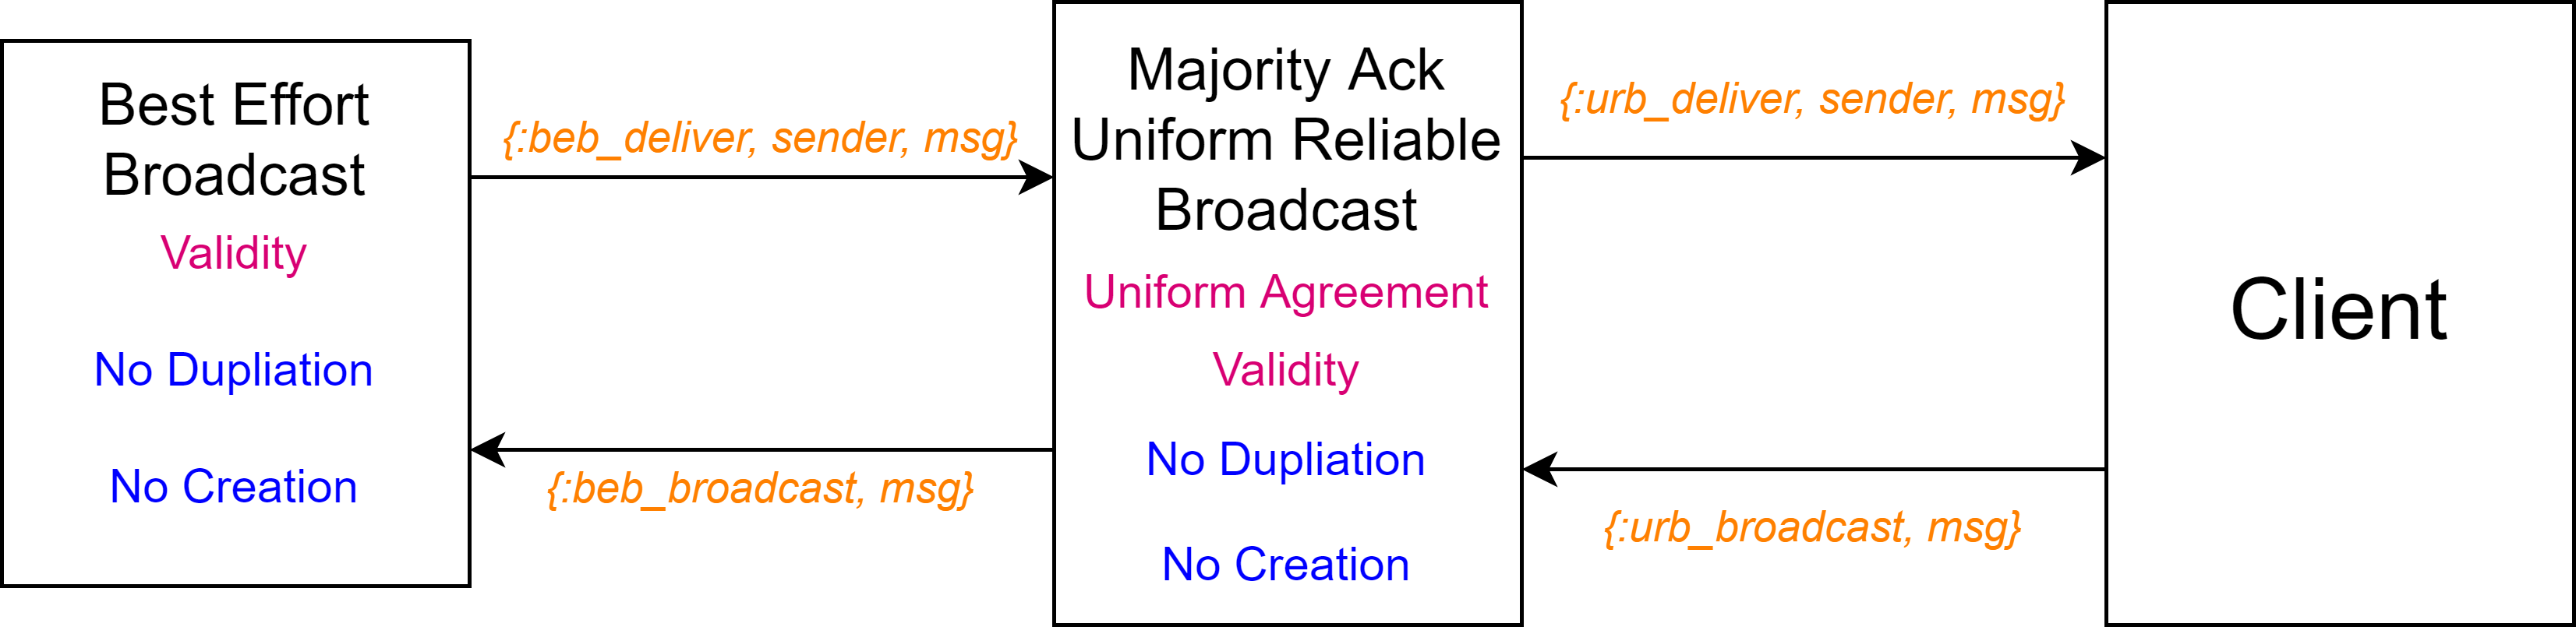
\includegraphics[width=.8\textwidth]{reliable_broadcast/images/majority_ack_uniform_reliable_broadcast.drawio.png}
    \end{center}
    \begin{itemize}
        \item \textit{Fail-silent} and does not use a \textit{failure detector}.
        \item If $n$ processes may crash, then $2n+1$ processes are needed with at least $n+1$ (majority) being correct
    \end{itemize}
\end{definitionbox}
\unfinished

